\documentclass[journal,12pt,twocolumn]{IEEEtran}
\usepackage{setspace}
\usepackage{gensymb}
\singlespacing
\usepackage[cmex10]{amsmath}
\usepackage{amsthm}
\usepackage{mathrsfs}
\usepackage{txfonts}
\usepackage{stfloats}
\usepackage{bm}
\usepackage{cite}
\usepackage{cases}
\usepackage{subfig}
\usepackage{longtable}
\usepackage{multirow}
\usepackage{enumitem}
\usepackage{mathtools}
\usepackage{steinmetz}
\usepackage{tikz}
\usepackage{circuitikz}
\usepackage{verbatim}
\usepackage{tfrupee}
\usepackage[breaklinks=true]{hyperref}
\usepackage{tkz-euclide}
\usetikzlibrary{calc,math}
\usepackage{listings}
    \usepackage{color}                                            %%
    \usepackage{array}                                            %%
    \usepackage{longtable}                                        %%
    \usepackage{calc}                                             %%
    \usepackage{multirow}                                         %%
    \usepackage{hhline}                                           %%
    \usepackage{ifthen}                                           %%
  %optionally (for landscape tables embedded in another document): %%
    \usepackage{lscape}     
\usepackage{multicol}
\usepackage{chngcntr}
\DeclareMathOperator*{\Res}{Res}
\renewcommand\thesection{\arabic{section}}
\renewcommand\thesubsection{\thesection.\arabic{subsection}}
\renewcommand\thesubsubsection{\thesubsection.\arabic{subsubsection}}

\renewcommand\thesectiondis{\arabic{section}}
\renewcommand\thesubsectiondis{\thesectiondis.\arabic{subsection}}
\renewcommand\thesubsubsectiondis{\thesubsectiondis.\arabic{subsubsection}}

% correct bad hyphenation here
\hyphenation{op-tical net-works semi-conduc-tor}
\def\inputGnumericTable{}                                 %%

\lstset{
frame=single, 
breaklines=true,
columns=fullflexible
}

\begin{document}


\newtheorem{theorem}{Theorem}[section]
\newtheorem{problem}{Problem}
\newtheorem{proposition}{Proposition}[section]
\newtheorem{lemma}{Lemma}[section]
\newtheorem{corollary}[theorem]{Corollary}
\newtheorem{example}{Example}[section]
\newtheorem{definition}[problem]{Definition}
\newcommand{\BEQA}{\begin{eqnarray}}
\newcommand{\EEQA}{\end{eqnarray}}
\newcommand{\define}{\stackrel{\triangle}{=}}

\bibliographystyle{IEEEtran}
\providecommand{\mbf}{\mathbf}
\providecommand{\pr}[1]{\ensuremath{\Pr\left(#1\right)}}
\providecommand{\qfunc}[1]{\ensuremath{Q\left(#1\right)}}
\providecommand{\sbrak}[1]{\ensuremath{{}\left[#1\right]}}
\providecommand{\lsbrak}[1]{\ensuremath{{}\left[#1\right.}}
\providecommand{\rsbrak}[1]{\ensuremath{{}\left.#1\right]}}
\providecommand{\brak}[1]{\ensuremath{\left(#1\right)}}
\providecommand{\lbrak}[1]{\ensuremath{\left(#1\right.}}
\providecommand{\rbrak}[1]{\ensuremath{\left.#1\right)}}
\providecommand{\cbrak}[1]{\ensuremath{\left\{#1\right\}}}
\providecommand{\lcbrak}[1]{\ensuremath{\left\{#1\right.}}
\providecommand{\rcbrak}[1]{\ensuremath{\left.#1\right\}}}
\theoremstyle{remark}
\newtheorem{rem}{Remark}
\newcommand{\sgn}{\mathop{\mathrm{sgn}}}
\providecommand{\abs}[1]{\left\vert#1\right\vert}
\providecommand{\res}[1]{\Res\displaylimits_{#1}} 
\providecommand{\norm}[1]{\left\lVert#1\right\rVert}
\providecommand{\mtx}[1]{\mathbf{#1}}
\providecommand{\mean}[1]{E\left[ #1 \right]}
\providecommand{\fourier}{\overset{\mathcal{F}}{ \rightleftharpoons}}
\providecommand{\system}{\overset{\mathcal{H}}{ \longleftrightarrow}}
\newcommand{\solution}{\noindent \textbf{Solution: }}
\newcommand{\cosec}{\,\text{cosec}\,}
\providecommand{\dec}[2]{\ensuremath{\overset{#1}{\underset{#2}{\gtrless}}}}
\newcommand{\myvec}[1]{\ensuremath{\begin{pmatrix}#1\end{pmatrix}}}
\newcommand{\mydet}[1]{\ensuremath{\begin{vmatrix}#1\end{vmatrix}}}
\numberwithin{equation}{subsection}
\makeatletter
\@addtoreset{figure}{problem}
\makeatother

\let\StandardTheFigure\thefigure
\let\vec\mathbf
\renewcommand{\thefigure}{\theproblem}



\def\putbox#1#2#3{\makebox[0in][l]{\makebox[#1][l]{}\raisebox{\baselineskip}[0in][0in]{\raisebox{#2}[0in][0in]{#3}}}}
     \def\rightbox#1{\makebox[0in][r]{#1}}
     \def\centbox#1{\makebox[0in]{#1}}
     \def\topbox#1{\raisebox{-\baselineskip}[0in][0in]{#1}}
     \def\midbox#1{\raisebox{-0.5\baselineskip}[0in][0in]{#1}}

\vspace{3cm}


\title{Assignment 1}
\author{Jaswanth Chowdary Madala}





% make the title area
\maketitle

\newpage

%\tableofcontents

\bigskip

\renewcommand{\thefigure}{\theenumi}
\renewcommand{\thetable}{\theenumi}


\begin{enumerate}
\item Two congruent circles intersect each other at points $\vec{A}$ and $\vec{B}$. Through $\vec{A}$ any line segment $\vec{PAQ}$ is drawn so that $\vec{P}$, $\vec{Q}$ lie on the two circles. Prove that $BP = BQ$.
\begin{figure}[ht]
\centering
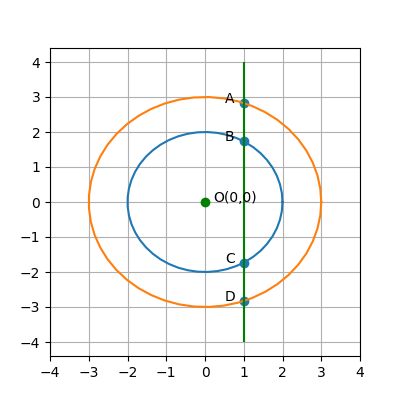
\includegraphics[width = \columnwidth]{"./figs/fig.png"}
\caption{Graph}
\label{fig:1}
\end{figure}

\textbf{Solution:}
Consider two congruent circles with radius $2\sqrt{2}$ with centres at $\myvec{2\\0}$, $\myvec{-2\\0}$. The equations of these circles is given by,
\begin{align}
\norm{\vec{x}}^2 + 2\vec{u_1}^\top\vec{x} + f_1 &= 0 
\label{eq:1}\\
\norm{\vec{x}}^2 + 2\vec{u_2}^\top\vec{x} + f_2 &= 0 
\label{eq:2}\\
\vec{u_1} = -\myvec{2\\0}, \, \vec{u_2} &= -\myvec{-2\\0}\\
f_1 = -4, \, f_2 &= -4
\end{align}
To get points of intersection $\vec{A}, \vec{B}$, the common chord of the circles is given by,
\begin{align}
2\vec{u_1}^\top\vec{x}-2\vec{u_2}^\top\vec{x}+f_1 - f_2 &= 0\\
\myvec{1&0}\vec{x} &= 0
\label{eq:3}
\end{align}
The equation \eqref{eq:3} can be written in parametric form as,
\begin{align}
\vec{h} = \myvec{0\\0}, \, \vec{m} = \myvec{0\\1}\\
\vec{x} = \myvec{0\\0} + \mu \myvec{0\\1}
\label{eq:4}
\end{align} 
The parameter $\mu$ of the points of intersection of line \eqref{eq:5} with the conic section \eqref{eq:6}
\begin{align}
\vec{x} &= \vec{h} + \mu \vec{m}
\label{eq:5}\\
\text{g}\brak{\vec{x}} &= \vec{x}^{\top}\vec{V}\vec{x}+2\vec{u}^{\top}\vec{x}+f=0
\label{eq:6}
\end{align}
is given by the equation 
\begin{align}
\mu^2\vec{m}^{\top}\vec{V}\vec{m} + 2 \mu\vec{m}^{\top}\brak{\vec{V}\vec{h}+\vec{u}} + \text{g}\brak{\vec{h}} &=0
\label{eq:7}
\end{align}
For the line to intersect the conic at 2 points, the discriminant of the quadratic equation \eqref{eq:6} should be greater than 0.
\begin{align}
\Delta &> 0\\
{\brak{\vec{m}^{\top}\brak{\vec{V}\vec{h}+\vec{u}}}}^2-\text{g}\brak{\vec{h}}\brak{\vec{m}^{\top}\vec{V}\vec{m}} &> 0
\end{align}
To find the points of intersection $\vec{A}, \vec{B}$, we find the intersection of the circle \eqref{eq:1}, common chord \eqref{eq:4}
\begin{align}
\vec{V} = \vec{I}, \, \vec{u} &= \myvec{-2\\0}, \, f = -4\\
\vec{h} = \myvec{0\\0}, \, \vec{m} &= \myvec{0\\1}\\
\vec{m}^{\top}\vec{V}\vec{m} &= 1\\
\vec{m}^{\top}\brak{\vec{V}\vec{h}+\vec{u}} &= 0\\
\text{g}\brak{\vec{h}} &= -4
\end{align}
Checking whether two circles intersect each other gives,
\begin{align}
{\brak{\vec{m}^{\top}\brak{\vec{V}\vec{h}+\vec{u}}}}^2-\text{g}\brak{\vec{h}}\brak{\vec{m}^{\top}\vec{V}\vec{m}} &= 0^2 - \brak{-4}\times1\\
&= 4
\end{align}
Hence, the two circles taken intersect each other.
\begin{align}
\mu^2 - 4 &=0\\
\mu &= \pm 2
\end{align}
From the equation \eqref{eq:4} the points $\vec{A},\vec{B}$ are given by,
\begin{align}
\vec{A} &= \myvec{0\\2}\\
\vec{B} &= \myvec{0\\-2} 
\end{align} 
Let us consider the direction vector, $\vec{m}$ of the line passing through the point $\vec{A}$ to be,
\begin{align}
\vec{m} = \myvec{2\\1}
\label{eq:8}
\end{align} 
The equation of the line passing through the point $\vec{A}$ with the direction vector \eqref{eq:8} in parametric form is given by,
\begin{align}
\vec{x} = \myvec{0\\2} + \mu \myvec{2\\1}
\label{eq:9}
\end{align}
Let $\vec{P}$ be the intersection of the line \eqref{eq:9} and the circle \eqref{eq:1}, $\vec{Q}$ be the intersection of the line \eqref{eq:9} and the circle \eqref{eq:2}. 

To find the point $\vec{P}$,
\begin{align}
\vec{V} = \vec{I}, \, \vec{u} &= \myvec{-2\\0}, \, f = -4\\
\vec{h} = \myvec{0\\2}, \, \vec{m} &= \myvec{2\\1}\\
\vec{m}^{\top}\vec{V}\vec{m} &= 5\\
\vec{m}^{\top}\brak{\vec{V}\vec{h}+\vec{u}} &= -2\\
\text{g}\brak{\vec{h}} &= 0 
\end{align}
Checking whether the line \eqref{eq:9} and circle \eqref{eq:1} intersect each other gives,
\begin{align}
{\brak{\vec{m}^{\top}\brak{\vec{V}\vec{h}+\vec{u}}}}^2-\text{g}\brak{\vec{h}}\brak{\vec{m}^{\top}\vec{V}\vec{m}} &= \brak{-2}^2 - \brak{0}\times5\\
&= 4
\end{align}
Hence, the line \eqref{eq:9} and circle \eqref{eq:1} intersect each other.
\begin{align}
5\mu^2 - 4 \mu &=0\\
\mu &= 0, \frac{4}{5}
\end{align}
\begin{align}
\vec{P} &= \myvec{\frac{8}{5}\\\\ \frac{14}{5}}
\end{align}
To find the point $\vec{Q}$,
\begin{align}
\vec{V} = \vec{I}, \, \vec{u} &= \myvec{2\\0}, \, f = -4\\
\vec{h} = \myvec{0\\2}, \, \vec{m} &= \myvec{2\\1}\\
\vec{m}^{\top}\vec{V}\vec{m} &= 5\\
\vec{m}^{\top}\brak{\vec{V}\vec{h}+\vec{u}} &= 6\\
\text{g}\brak{\vec{h}} &= 0
\end{align}
Checking whether the line \eqref{eq:9} and circle \eqref{eq:2} intersect each other gives,
\begin{align}
{\brak{\vec{m}^{\top}\brak{\vec{V}\vec{h}+\vec{u}}}}^2-\text{g}\brak{\vec{h}}\brak{\vec{m}^{\top}\vec{V}\vec{m}} &= 6^2 - \brak{0}\times5\\
&= 36
\end{align}
Hence, the line \eqref{eq:9} and circle \eqref{eq:1} intersect each other.
\begin{align}
5\mu^2 + 12 \mu &=0\\
\mu &= 0, -\frac{12}{5}\\
\vec{Q} &= \myvec{-\frac{24}{5}\\\\-\frac{2}{5}}\\
\norm{\vec{B}-\vec{P}} &= \norm{\myvec{0\\\\-2} - \myvec{\frac{8}{5}\\\\ \frac{14}{5}}}\\
&= \norm{\myvec{-\frac{8}{5}\\\\-\frac{24}{5}}}\\
&= \frac{8\sqrt{10}}{5}\\
\norm{\vec{B}-\vec{Q}} &= \norm{\myvec{0\\\\-2} - \myvec{-\frac{24}{5}\\\\-\frac{2}{5}}}\\
&= \norm{\myvec{\frac{24}{5}\\\\-\frac{8}{5}}}\\
&= \frac{8\sqrt{10}}{5}
\end{align}
Hence, $BP = BQ$.
The parameters used in the construction are shown in the below table \ref{tab:1}

\begin{table}[h]
\centering
%%%%%%%%%%%%%%%%%%%%%%%%%%%%%%%%%%%%%%%%%%%%%%%%%%%%%%%%%%%%%%%%%%%%%%
%%                                                                  %%
%%  This is a LaTeX2e table fragment exported from Gnumeric.        %%
%%                                                                  %%
%%%%%%%%%%%%%%%%%%%%%%%%%%%%%%%%%%%%%%%%%%%%%%%%%%%%%%%%%%%%%%%%%%%%%%

\begin{center}
\begin{tabular}{|c|c|c|}
\hline
\textbf{RV}& \textbf{Values} & \textbf{Description} \\ \hline
$X$		   & 	$\{0,1\}$	&  1st draw - 0: black card, 1: red card\\ \hline
$Y$ 		   & 	$\{0,1\}$	&  2nd draw - 0: black card, 1: red card\\ \hline
$X,Y$ 		   & 	$\{00\}$	&	2 cards drawn are black\\ \hline
\end{tabular}
\end{center}

\caption{}
\label{tab:1}
\end{table}
\end{enumerate}
\end{document}



